\documentclass{article}
\usepackage[utf8]{inputenc}
\usepackage{graphicx}

\title{Informe Parcial II}
\author{daniel.perez19 }
\date{September 2021}

\begin{document}

\begin{titlepage}
    \begin{center}
        \vspace*{1cm}
            
        \Huge
        \textbf{Informe Parcial 2}
            
        \vspace{0.5cm}
        \LARGE
        Informática II
            
        \vspace{1.5cm}
            
        \textbf{Daniel Perez Gallego CC. 1193088770\\Jorge Montaña Cisneros CC.  1007327968}
            
        \vfill
            
        \vspace{0.8cm}
            
        \Large
        Departamento de Ingeniería Electrónica y Telecomunicaciones\\
        Universidad de Antioquia\\
        Medellín\\
        Septiembre de 2021
            
    \end{center}
\end{titlepage}

\tableofcontents

\section{Análisis}
\subsection{Análisis del problema}
Al analizar detenidamente el parcial y las instrucciones planteadas, observamos que el mayor reto consistiría en la modificación del tamaño de las imágenes, adaptándolo a un tamaño específico, ya sea aumentando o disminuyendo la proporción.\\ 
\\Para el submuestreo, pensamos a forma de solución organizar los RGB en filas y columnas separadas, una vez hecho esto, eliminar las que son pares, de este modo, tendremos la misma imagen, pero recortada a un cuarto de la,  obteniendo un tamaño menor pero proporcional a la imagen original, repiendo el proceso hasta obtener el tamaño deseado.\\

Si la imagen dada tiene un tamaño menor al esperado, se hará un proceso parecido al de eliminar, pero en este caso se aumentarán las filas/columnas colocandolas continuas a ellas mismas  hasta quedar con la proporción deseada.

En el caso de que la imagen no se adapte al tamaño específico deseado, se va a eliminar/aunmentar ya sea las filas o columnas sobrantes o faltantes de los extremos para que tenga una propoción adecuada.\\
\\Mientras más pequeña sea la matriz de LEDs, menos información deberemos exportar, será más eficiente y fácil, sin embargo, la imagen se volverá dificil de reconocer para el usuario, por lo tanto, acordamos hacer la matriz de LEDs de 16x16\\

Para el código, pensamos realizar un vector de 3 dimensiones, para la organización de los pixeles RGB, despúes pensamos en usar otro vector de 3 dimensiones dónde se hará una reducción de filas y columnas. Finalmente, para que quede listo para el programa de tinkercad \\

Para las clases, usaremos una que nos entregue los píxeles RGB y lo entregue en contenedores. Otra clase para eliminar/duplicar filas y columnas además, una clase para eliminar/agregar las filas/columnas en los extremos para llegar al tamaño de la matriz deseado. Y para finalizar, otra clase para convertir las variables a string y con esto último, generar un .txt


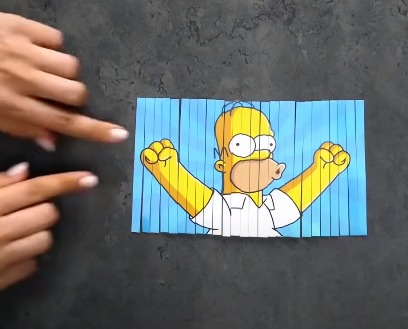
\includegraphics[width=4cm]{Imagenes/recorte1.jpeg}
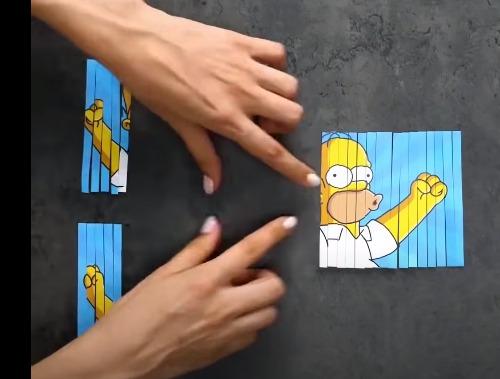
\includegraphics[width=4cm]{Imagenes/recorte2.jpeg}
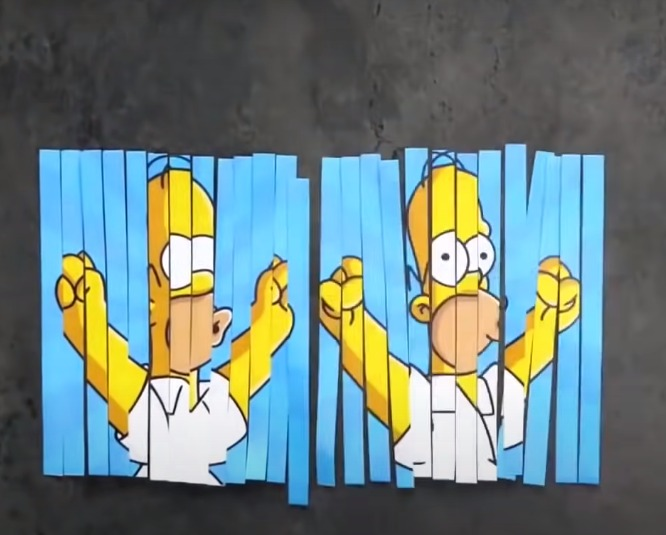
\includegraphics[width=4cm]{Imagenes/recorte3.jpeg}
\vspace{0,3cm}

\subsection{Tareas a realizar}
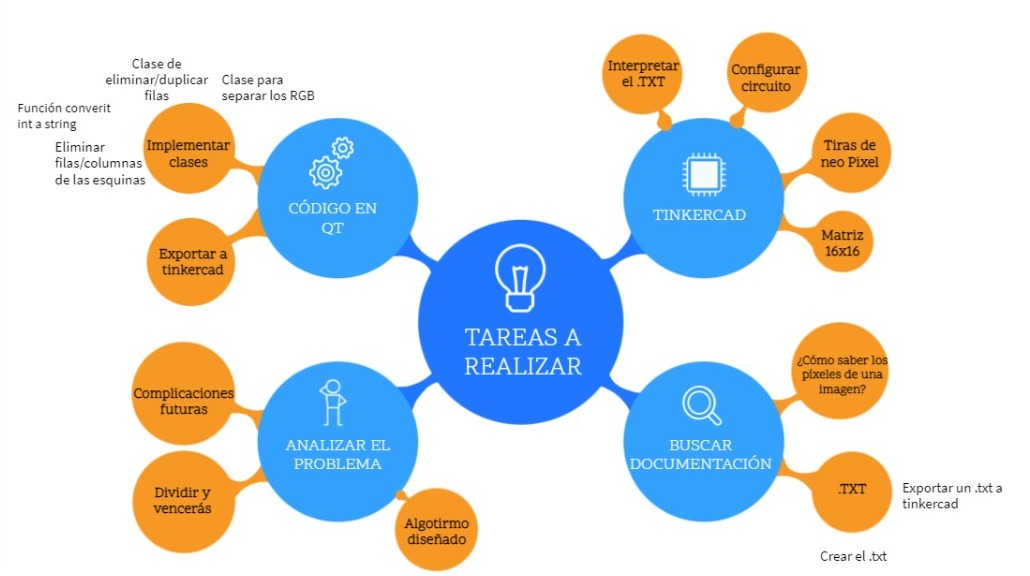
\includegraphics[width=15cm]{Imagenes/Esquema.jpeg}

\subsection{Algoritmo implementado}
Diagrama de flujo del algoritmo que implemenatremos para la solución del problema (No código)\\
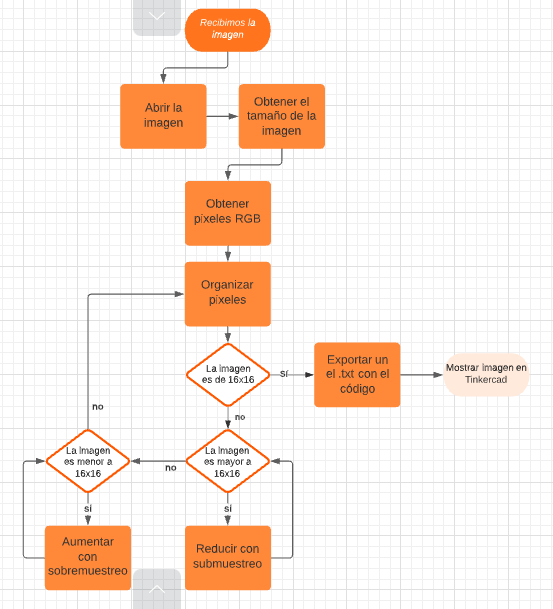
\includegraphics[width=12cm]{Imagenes/Algo.png}

\subsection{Consideraciones}
Una de las consideraciones más importantes que encontramos fué una correcta identificación de cada columna y fila de píxeles RGB, y mirar el modo de separar cada una.\\
El método para generar el .txt final y enviarlo a tinkercad.\\



\section{Clases implementadas}
1. Sobremuestreo
2. Submuestreo
3. Lectura y escritura
4. Correccción

\section{Esquema de las clases}

\section{Código}
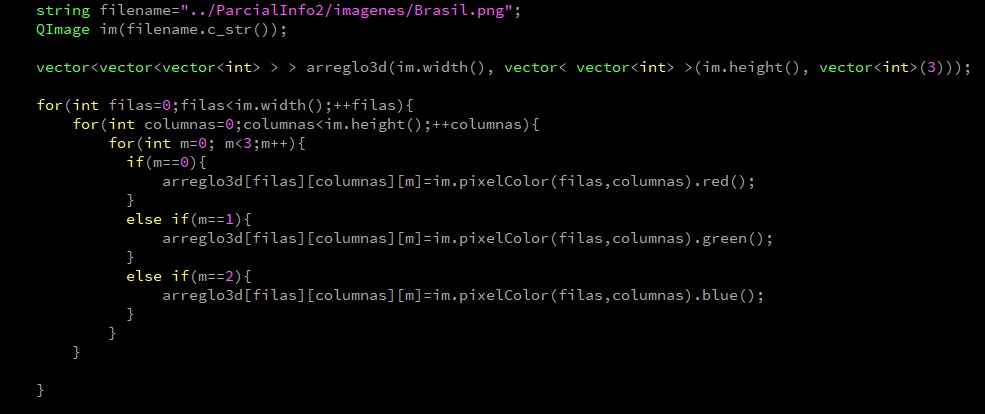
\includegraphics[width=10cm]{Imagenes/Codigo_1.jpeg}


\section{Estructura del circuito montado}
Nuestro primer diseño de la matriz de LEDs en Tinkerdad, el cual pensamos realizarla de 16x16\\
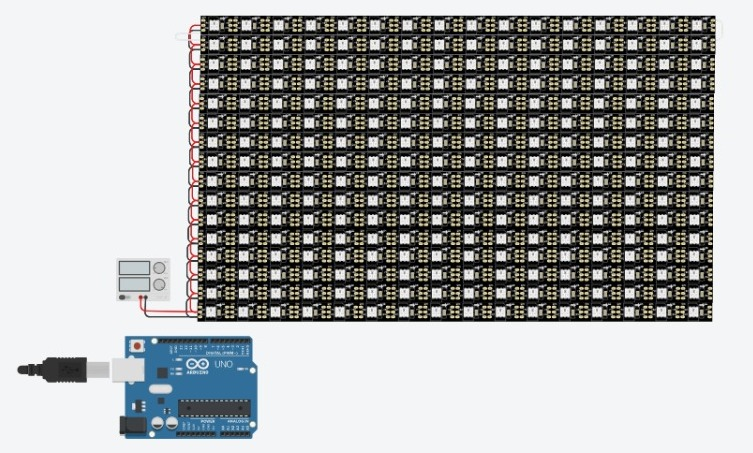
\includegraphics[width=10cm]{Imagenes/circuito_1.jpeg}

\section{Problemas presentados}







\end{document}
